\documentclass{article}
\usepackage[T1]{fontenc}
\usepackage{graphicx}
\usepackage{amsmath, amsthm, amssymb}
\usepackage{hyperref}
\usepackage{polski}
\usepackage{array}
\usepackage{float}
\newtheorem{theorem}{Twierdzenie}
\usepackage[a4paper, left=1.5cm, right=3cm, top=2cm, bottom=2cm]{geometry}
\theoremstyle{definition}
\usepackage{enumerate}
\usepackage{listings}
\usepackage{color}
\newtheorem{definition}{Definicja}

\title{Sprawozdanie Lista3}
\author{Paweł Solecki}
\date{\today}
\begin{document}
	\maketitle
	\section{Zadanie 1: Quick\_Sort}
	Zaimplementuj algorytm CUT\_ROD w wersji naiwnej, ze spamietywaniem oraz iteracyjnej.
	\begin{lstlisting}[language=C++, tabsize=3, caption={Implementacja CUT\_ROD}]
		int CUT_ROD(int p[], int n) {
			if (n == 0) return 0;
			int q = -1;
			for (int i = 1; i <= n; i++) {
				q = max(q, p[i] + CUT_ROD(p, n - i));
			}
			return q;
		}
	\end{lstlisting}
	
	\begin{lstlisting}[language=C++, tabsize=3, caption={Implementacja MEMORIZED\_CUT\_ROD}]
		int MEMORIZED_CUT_ROD_AUX(int p[], int n, int r[], int s[]) {
			if (r[n] >= 0) return r[n];
			int q = (n == 0) ? 0 : -1;
			for (int i = 1; i <= n; i++) {
				int current_value = p[i] + MEMORIZED_CUT_ROD_AUX(p, n - i, r, s);
				if (q < current_value) {
					q = current_value;
					s[n] = i;
				}
			}
			r[n] = q;
			return q;
		}
		
		int MEMORIZED_CUT_ROD(int p[], int n, int s[]) {
			int r[n + 1];
			memset(r, -1, sizeof(r));
			return MEMORIZED_CUT_ROD_AUX(p, n, r, s);
	\end{lstlisting}
	
	\begin{lstlisting}[language=C++, tabsize=3, caption={Implementacja ITER\_CUT\_ROD}]
		void ITER_CUT_ROD(int p[], int n, int r[], int s[]) {
			r[0] = 0;
			for (int j = 1; j <= n; j++) {
				int q = -1;
				for (int i = 1; i <= j; i++) {
					if (q < p[i] + r[j - i]) {
						q = p[i] + r[j - i];
						s[j] = i;
					}
				}
				r[j] = q;
			}
		}
	\end{lstlisting}
	\section{Zadanie 2: LCS}
	Zaimplementuj algorytm LCS w wersji rekurencyjnej ze spamietywaniem oraz w wersji
	iteracyjnej.
	\begin{lstlisting}[language=C++, tabsize=3, caption={Implementacja LCS\_RECURSIVE}]
		int LCS_RECURSIVE(const string& a, const string& b, int m, int n, int** memo) {
			if (m == 0 || n == 0) {
				return 0;
			}
			if (memo[m][n] != -1) {
				return memo[m][n];
			}
			if (a[m - 1] == b[n - 1]) {
				return memo[m][n] = 1 + LCS_RECURSIVE(a, b, m - 1, n - 1, memo);
			}
			return memo[m][n] = max(LCS_RECURSIVE(a, b, m - 1, n, memo),
			LCS_RECURSIVE(a, b, m, n - 1, memo));
		}
	\end{lstlisting}
	
	\begin{lstlisting}[language=C++, tabsize=3, caption={Implementacja LCS\_ITERATIVE}]
		char** LCS_ITERATIVE(const string& a, const string& b, int& lcsLength) {
			int lenA = a.length();
			int lenB = b.length();
			
			int** dp = new int*[lenA + 1];
			char** d = new char*[lenA + 1];
			for (int i = 0; i <= lenA; i++) {
				dp[i] = new int[lenB + 1];
				d[i] = new char[lenB + 1];
			}
			
			for (int i = 0; i <= lenA; i++) dp[i][0] = 0;
			for (int j = 0; j <= lenB; j++) dp[0][j] = 0;
			
			for (int i = 1; i <= lenA; i++) {
				for (int j = 1; j <= lenB; j++) {
					if (a[i - 1] == b[j - 1]) {
						dp[i][j] = dp[i - 1][j - 1] + 1;
						d[i][j] = '\\';
					} else if (dp[i - 1][j] >= dp[i][j - 1]) {
						dp[i][j] = dp[i - 1][j];
						d[i][j] = '|';
					} else {
						dp[i][j] = dp[i][j - 1];
						d[i][j] = '-';
					}
				}
			}
			
			lcsLength = dp[lenA][lenB];
			
			for (int i = 0; i <= lenA; i++) {
				delete[] dp[i];
			}
			delete[] dp;
			
			return d;
		}
	\end{lstlisting}
	\section{Zadanie 3: ACTIVITY\_SELECTOR}
	Zaimplementuj algorytm ACTIVITY\_SELECTOR w wersji rekurencyjnej i iteracyjnej. Zmodyfikuj go tak, by działał na danych wejściowych posortowanych względem czasu rozpoczęcia. Napisz "konkurencyjny"kod oparty na programowaniu dynamicznym.
	\begin{lstlisting}[language=C++, tabsize=3, caption={Implementacja rekurencji bez modyfikacji}]
		void Rec_1(int p[], int k[], int n, int current, int zajecia[], int &ile) {
			int next = current + 1;
			while (next <= n && p[next] < k[current]) {
				next++;
			}
			if (next <= n) {
				zajecia[ile++] = next;
				Rec_1(p, k, n, next, zajecia, ile);
			}
		}
	\end{lstlisting}
	\begin{lstlisting}[language=C++, tabsize=3, caption={Implementacja iteracji bez modyfikacji}]
		void Iter_1(int p[], int k[], int n, int zajecia[], int &ile) {
			zajecia[ile++] = 1;
			int current = 1;
			
			for (int next = 2; next <= n; next++) {
				if (p[next] >= k[current]) {
					zajecia[ile++] = next;
					current = next;
				}
			}
		}
	\end{lstlisting}
	\begin{lstlisting}[language=C++, tabsize=3, caption={Implementacja rekurencji z modyfikacją}]
		void Rec_2(int p[], int k[], int current, int zajecia[], int &ile) {
			int prev = current - 1;
			while (prev > 0 && k[prev] > p[current]) {
				prev--;
			}
			if (prev > 0) {
				zajecia[ile++] = prev;
				Rec_2(p, k, prev, zajecia, ile);
			}
		}
	\end{lstlisting}
	\begin{lstlisting}[language=C++, tabsize=3, caption={Implementacja iteracji z modyfikacją}]
		void Iter_2(int p[], int k[], int n, int zajecia[], int &ile) {
			zajecia[ile++] = n - 1;
			int current = n - 1;
			
			for (int prev = n - 2; prev >= 1; prev--) {
				if (k[prev] <= p[current]) {
					zajecia[ile++] = prev;
					current = prev;
				}
			}
		}
	\end{lstlisting}
	\begin{lstlisting}[language=C++, tabsize=3, caption={Implementacja wersji opartej na programowaniu dynamicznym}]
		void Dyn(int p[], int k[], int n) {
			int** c = new int*[n + 2];
			int** b = new int*[n + 2];
			
			for (int i = 0; i < n + 2; ++i) {
				c[i] = new int[n + 2]{0};
				b[i] = new int[n + 2]{0};
			}
			
			for (int length = 2; length <= n + 1; ++length) {
				for (int i = 0; i <= n - length + 1; ++i) {
					int j = i + length;
					
					for (int m = j - 1; m > i; --m) {
						if (k[i] <= p[m] && k[m] <= p[j] &&
						c[i][m] + c[m][j] + 1 > c[i][j]) {
							c[i][j] = c[i][m] + c[m][j] + 1;
							b[i][j] = m;
						}
					}
				}
			}
			
			cout << "Maksymalna liczba zajec: " << c[0][n + 1] << endl;
			
			for (int i = 0; i < n + 2; ++i) {
				delete[] c[i];
				delete[] b[i];
			}
			delete[] c;
			delete[] b;
		}
	\end{lstlisting}
	\section{Zadanie 4: test CUT\_ROD}
	Pierwsza tabela przedstawia czas działania naiwnej wersji CUT\_ROD dla różnych długości pręta.
		\begin{table}[h]
		\centering
		\resizebox{0.3\textwidth}{!}{
			\begin{tabular}{|c|c|}
				\hline
				\textbf{Rozmiar pręta} & \textbf{Czas (s)} \\ \hline
				5                     & 0.001097          \\ \hline
				10                    & 0.00036           \\ \hline
				15                    & 0.001169          \\ \hline
				20                    & 0.020682          \\ \hline
				25                    & 0.375936          \\ \hline
			\end{tabular}
		}
		\caption{Czas wykonania CUT\_ROD}
	\end{table}
	Druga tabela wraz z wykresem stanowi porównanie wersji ze spamiętywaniem z wersją iteracyjną.
	\begin{table}[H]
		\centering
		\resizebox{\textwidth}{!}{
			\begin{tabular}{|c|c|c|}
				\hline
				\textbf{Rozmiar pręta} & \textbf{Czas (s) ze spamiętywaniem} & \textbf{Czas (s) iteracyjna} \\ \hline
				50                     & 0.003259                       & 0.003344                     \\ \hline
				100                    & 0.018038                       & 0.019652                     \\ \hline
				200                    & 0.033822                       & 0.044269                     \\ \hline
				400                    & 0.143111                       & 0.155705                     \\ \hline
				800                    & 0.278268                       & 0.302285                     \\ \hline
				1000                   & 0.301191                       & 0.304254                     \\ \hline
		\end{tabular}}
		\caption{Porównanie czasu wykonania metodą ze spamiętywaniem i iteracyjną.}
		\label{tab:czas_wykonania}
	\end{table}
	\begin{figure}[H]	
		\centering
		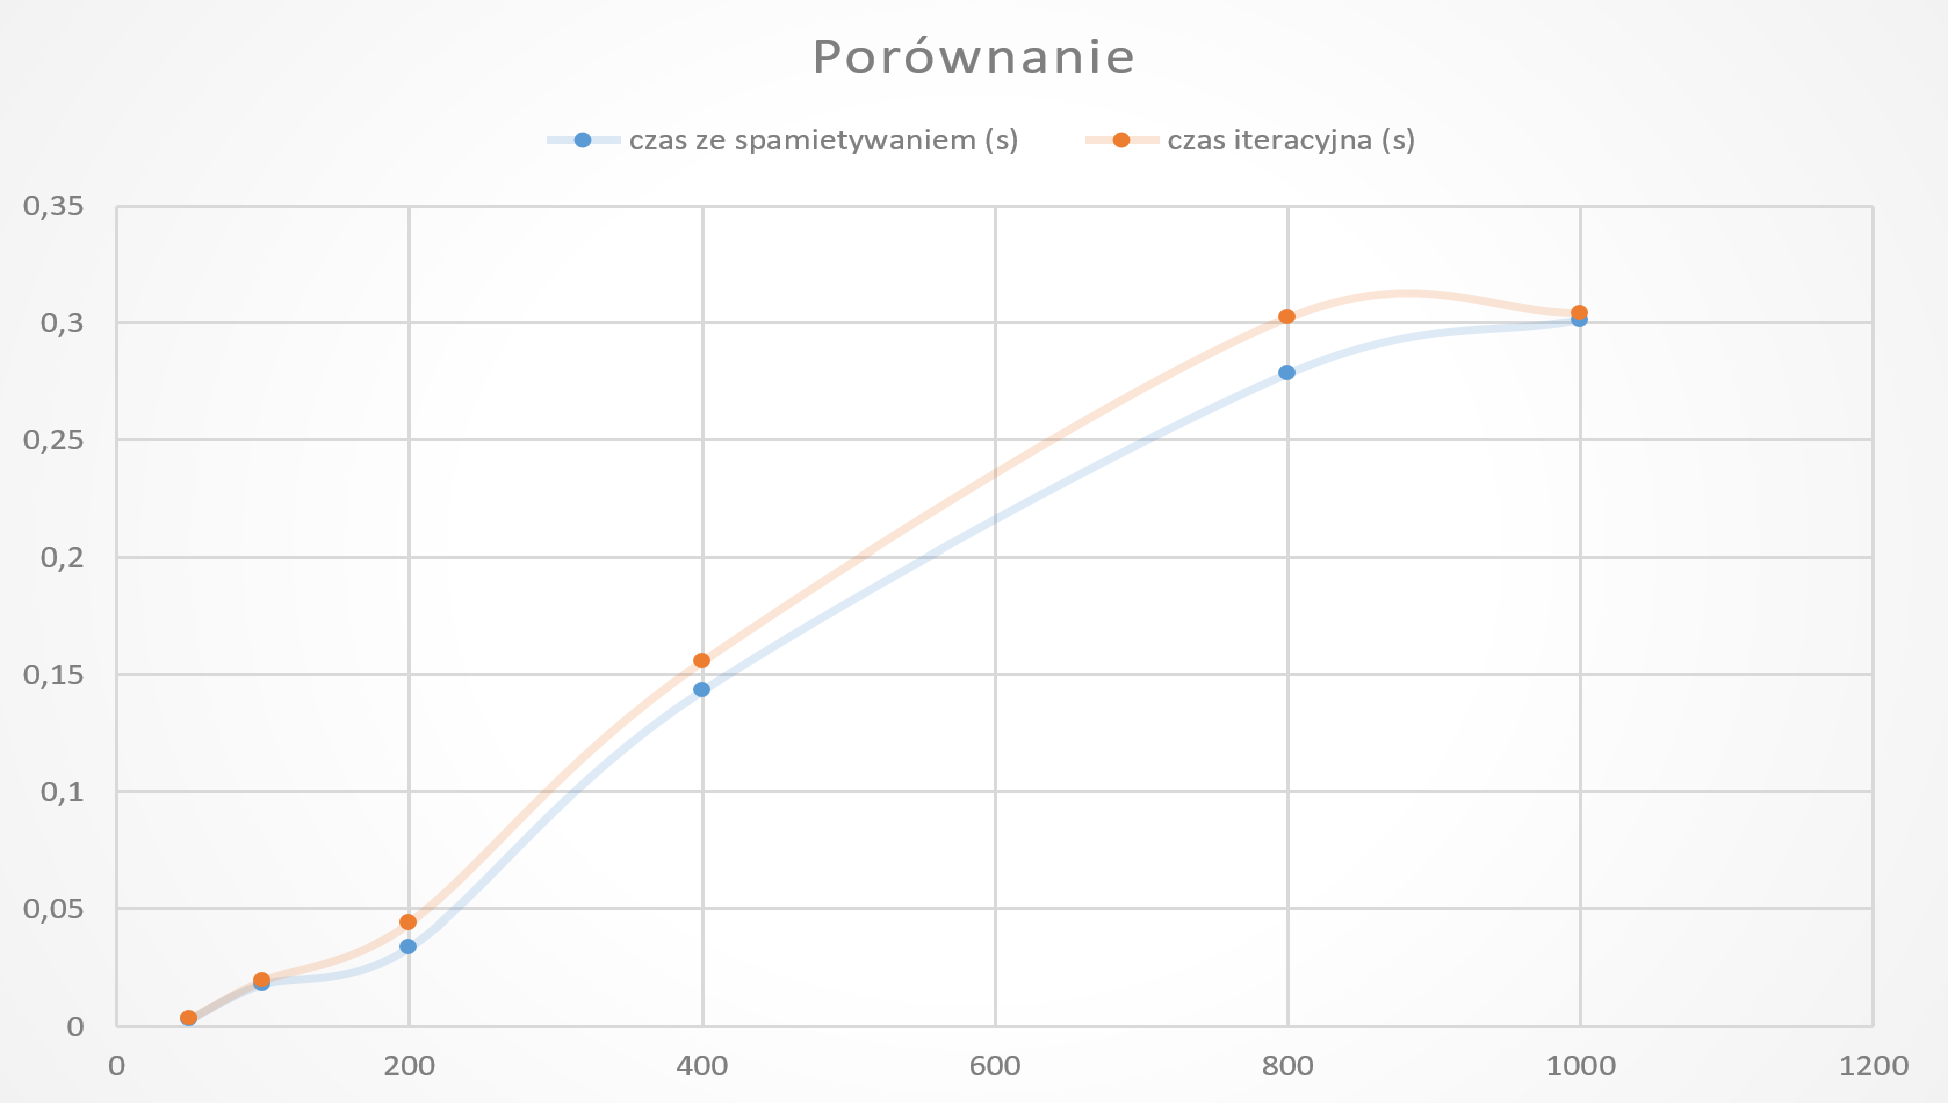
\includegraphics[width=1.0\textwidth]{w2.png} 
	\end{figure}
	\textbf{Wnioski:} Naiwna metoda rekurencyjna (CUT\_ROD) charakteryzuje się wykładniczą złożonością obliczeniową, co powoduje, że czas wykonania gwałtownie rośnie wraz ze wzrostem długości pręta. Jak pokazują wyniki w tabelach, dla długości pręta większych niż 15 algorytm ten staje się niepraktyczny, a dla większych danych wejściowych (np. długości 50 i więcej) jego czas działania jest nie do przyjęcia. Metoda ta, mimo swojej prostoty, może być stosowana jedynie  dla bardzo małych danych.
	
	Znacznie lepsze wyniki zapewnia metoda z pamiętaniem (MEMORIZED\_CUT\_ROD), która dzięki wykorzystaniu mechanizmu memoizacji eliminuje powtarzające się obliczenia. Dzięki temu algorytm ten jest w stanie efektywnie działać nawet dla dużych długości prętów, takich jak 800 czy 1000, co zostało potwierdzone przez uzyskane czasy wykonania w tabelach. Metoda iteracyjna (ITER\_CUT\_ROD) ma zbliżoną złożoność obliczeniową osiąga podobne czasy działania, choć nieco wyższe w porównaniu do metody z pamiętaniem, co wynika z dodatkowych iteracji przeglądających wszystkie podproblemy. Oba podejścia – ze spamiętywaniem i iteracyjne – pozwalają uzyskać tę samą maksymalną cenę oraz optymalny podział pręta, co potwierdza poprawność ich implementacji.
	
	Podsumowując, naiwna metoda rekurencyjna jest niewydajna i nie nadaje się do praktycznych zastosowań. Metoda ze spamiętywaniem i algorytm iteracyjny są efektywnymi rozwiązaniami, które zapewniają odpowiednie czasy wykonania nawet dla dużych długości prętów. W praktycznych zastosowaniach wybór między tymi metodami może zależeć od preferencji implementacyjnych, przy czym algorytm iteracyjny jest często preferowany ze względu na swoją prostszą strukturę. 
	\section{Zadanie 5:  Porównanie działania LCS\_RECURSIVE i LCS\_ITERATIVE}
	Wykres i tabela przedstawiają czas działania obu algorytmów dla różnej długości ciągów liter.
	\begin{table}[H]
		\centering
		\begin{tabular}{|c|c|c|}
			\hline
			\textbf{Długość ciągu} & \textbf{Rekurencyjna (s)} & \textbf{Iteracyjna (s)} \\ \hline
			500  & 0.022411 & 0.009585 \\ \hline
			1000 & 0.074994 & 0.046722 \\ \hline
			2000 & 0.241514 & 0.127017 \\ \hline
			4000 & 0.888453 & 0.284605 \\ \hline
			8000 & 2.46350  & 1.06778  \\ \hline
			10000 & 3.19382  & 1.63913  \\ \hline
		\end{tabular}
		\caption{Porównanie czasu wykonania algorytmu rekurencyjnego i iteracyjnego dla różnych długości ciągów.}
		\label{tab:czas_algorytmy}
	\end{table}
	\begin{figure}[H]	
		\centering
		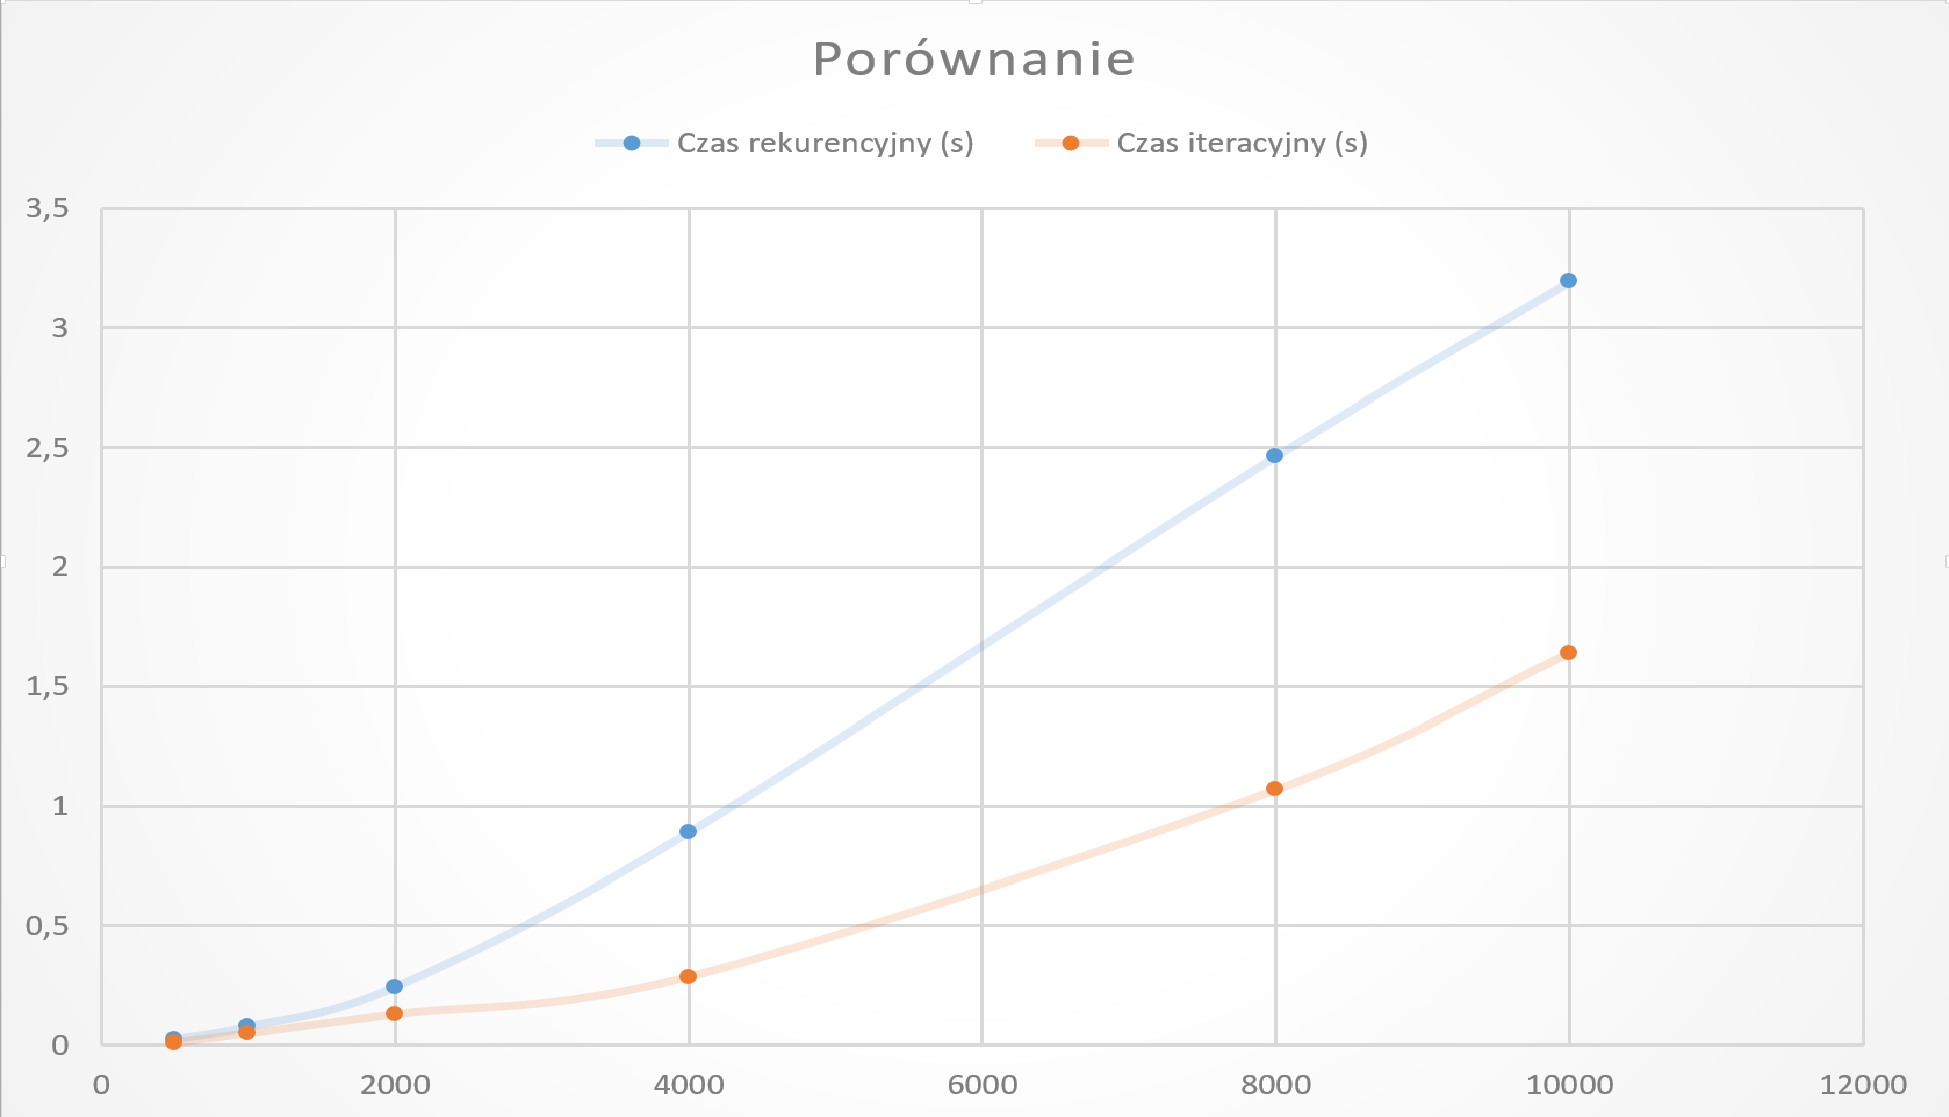
\includegraphics[width=1.0\textwidth]{w1.png} 
	\end{figure}
	\textbf{Wnioski:}Wyniki testów czasowych dla algorytmów rekurencyjnego i iteracyjnego do znajdowania najdłuższego wspólnego podciągu (LCS) pokazują, że algorytm iteracyjny jest znacznie szybszy. Czas wykonania algorytmu rekurencyjnego rośnie szybko w miarę zwiększania długości ciągów, osiągając 3.19 sekundy dla ciągu o długości 10000, podczas gdy algorytm iteracyjny potrzebuje tylko 1.64 sekundy. Choć wersja rekurencyjna z memoizacją poprawia wydajność, to algorytm iteracyjny jest bardziej wydajny i lepiej skaluje się przy większych danych.
	\section{Zadanie 6: Porównanie algorytmów ACTIVITY\_SELECTOR}
	Pierwsza tabela i wykres przedstawiają czasy działania algorytmów iteracyjnych i rekurencyjnych ( wraz z modyfikacjami) w zależności od n.
	\begin{table}[H]
		\centering
		\begin{tabular}{|c|c|c|c|c|}
			\hline
			\textbf{n} & \textbf{Rec\_1} & \textbf{Iter\_1} & \textbf{Rec\_2} & \textbf{Iter\_2} \\ \hline
			500  & 0.000003 & 0.000003 & 0.000004 & 0.000005 \\ \hline
			1000 & 0.000006 & 0.000007 & 0.000028 & 0.000010 \\ \hline
			2000 & 0.000014 & 0.000016 & 0.000041 & 0.000016 \\ \hline
			4000 & 0.000033 & 0.000024 & 0.000051 & 0.000046 \\ \hline
			8000 & 0.000058 & 0.000040 & 0.000086 & 0.000066 \\ \hline
			10000 & 0.000082 & 0.000067 & 0.000095 & 0.000091 \\ \hline
		\end{tabular}
		\caption{Czasy (s) dla Rec\_1, Iter\_1, Rec\_2, Iter\_2 for various n}
	\end{table} 
	\begin{figure}[H]	
		\centering
		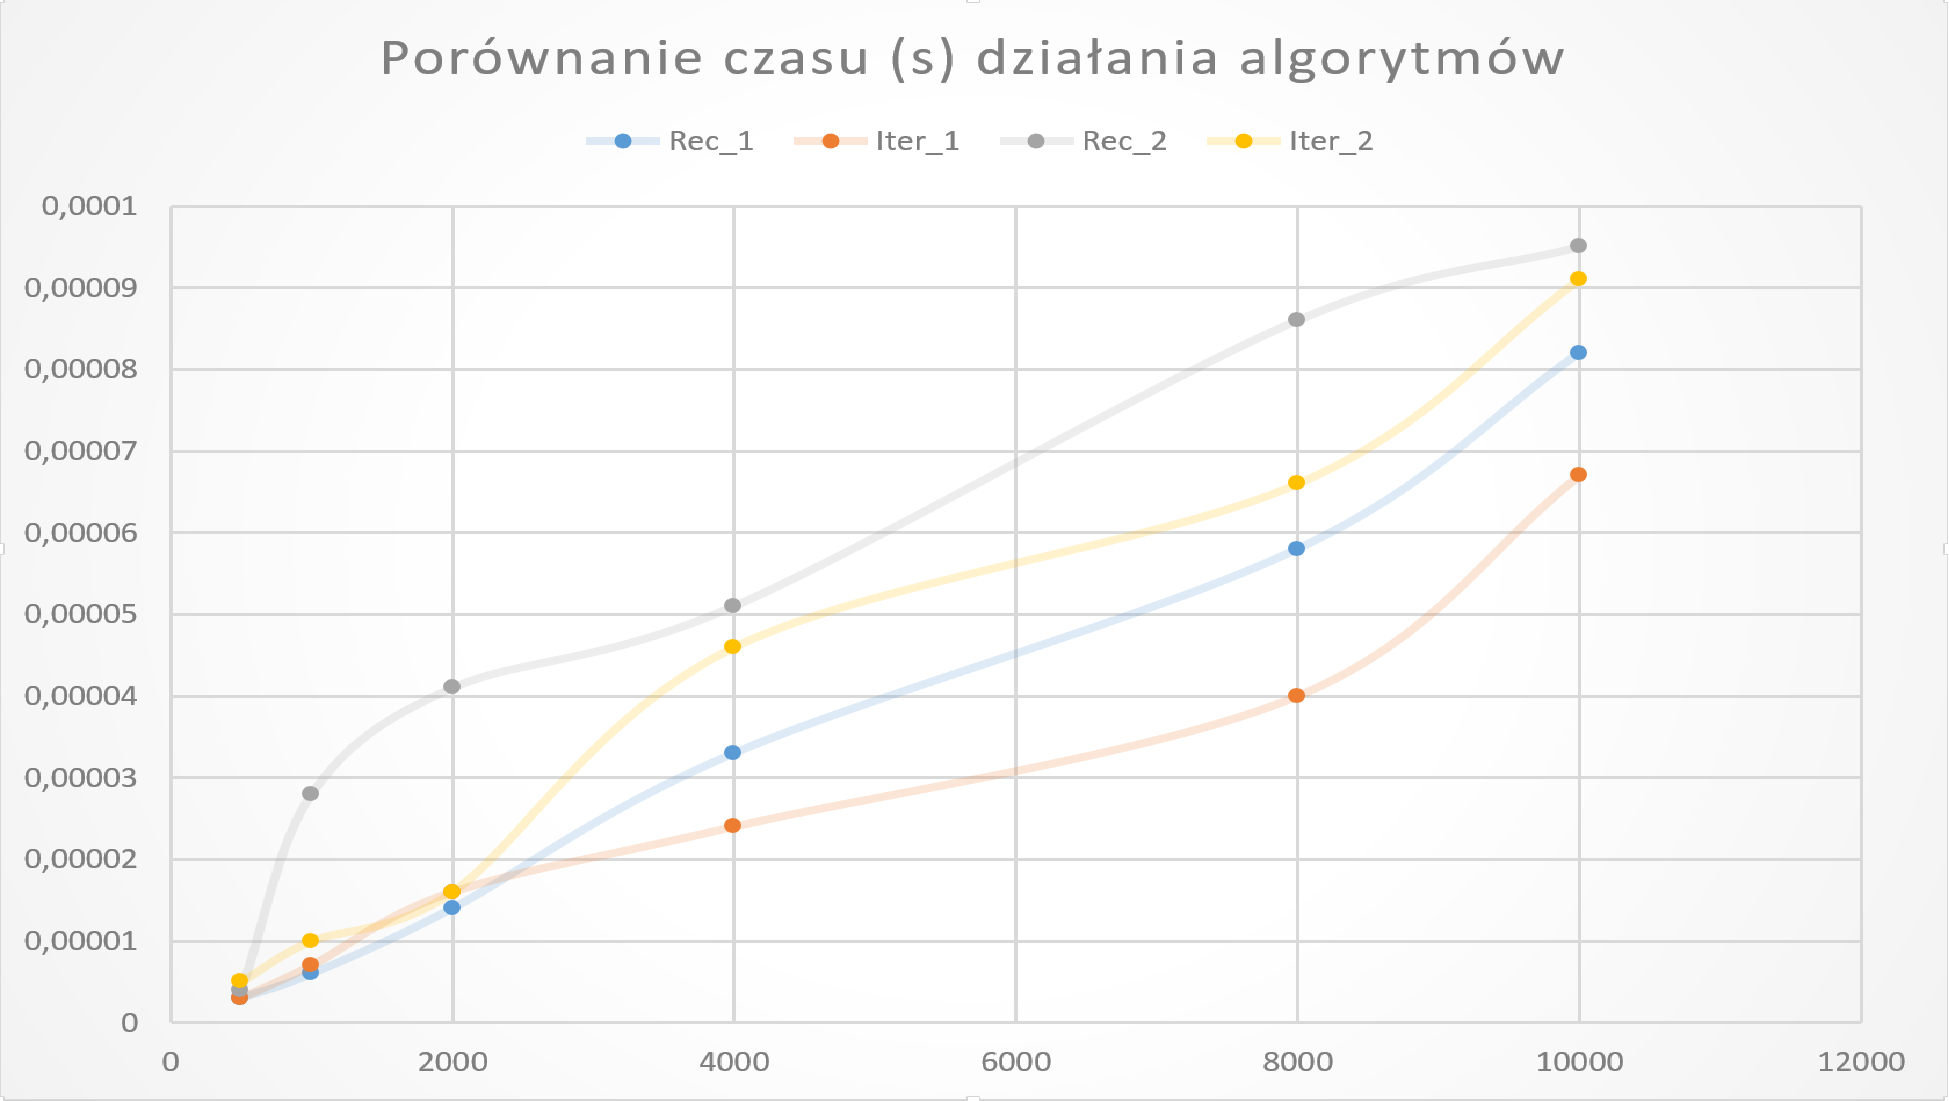
\includegraphics[width=1.0\textwidth]{w3.png} 
	\end{figure}
	Druga tabela przedstawia czasy działania "konkurencyjnego" kodu opartego na programowaniu dynamicznym.
	\begin{table}[H]
		\centering
		\begin{tabular}{|c|c|}
			\hline
			\textbf{n} & \textbf{Dyn (s)} \\ \hline
			500  & 0.369595 \\ \hline
			1000 & 3.331569 \\ \hline
			2000 & 22.409703 \\ \hline
			4000 & 319.915037 \\ \hline
		\end{tabular}
		\caption{kod oparty na programowaniu dynamicznym}
	\end{table}
	\textbf{Wnioski:}Na podstawie wyników czasów wykonania algorytmów dla różnych wartości n można zauważyć, że algorytmy rekurencyjne (Rec\_1, Rec\_2) oraz iteracyjne (Iter\_1, Iter\_2) mają podobne czasy wykonania, które rosną w sposób nieliniowy wraz ze wzrostem n, ale pozostają na stosunkowo niskim poziomie (mikrosekundy) nawet dla dużych danych (n do 10000). Z kolei algorytm oparty na programowaniu dynamicznym (Dyn) charakteryzuje się znacznie większymi czasami wykonania, które rosną wykładniczo przy większych n. Dla n = 500 czas wynosi 0.37 sekundy, a dla n = 10000 aż 319.92 sekundy. W praktyce, dla n do 10000, algorytmy rekurencyjne i iteracyjne są bardziej wydajne, a algorytm dynamiczny jest znacznie wolniejszy, mimo potencjalnych korzyści w bardziej złożonych problemach. Algorytmy rekurencyjne i iteracyjne są zatem bardziej odpowiednie dla tego zadania, zwłaszcza przy mniejszych i średnich danych.
\end{document}